\documentclass[pageno]{jpaper}

%------------------------------------------------------------------------------
%                                  Preamble. 
%------------------------------------------------------------------------------
%
\usepackage{times}
\usepackage[normalem]{ulem}
%\usepackage{txfonts}
\usepackage{url}
\usepackage{tikz}
%\usepackage{ifpdf}
\usepackage{color}
%\usepackage{pifont}
\usepackage{fancyhdr}
\usepackage{graphicx}
\usepackage{hyphenat}
%\usepackage{titlesec}
\usepackage[authoryear,square,comma,sort&compress]{natbib}

% Use a smaller font size for URLs:
\makeatletter
\def\url@myurlstyle{%
   \@ifundefined{selectfont}{\def\UrlFont{\sf}}{\def\UrlFont{\sf}}}
   \makeatother
\urlstyle{myurl}

% Section names, figure names and algorithm names.
\renewcommand{\tableautorefname}{Table}
\renewcommand{\figureautorefname}{Figure}
\renewcommand{\sectionautorefname}{Section}
\renewcommand{\subsectionautorefname}{Section}
\renewcommand{\subsubsectionautorefname}{Section}
\newcommand{\figref}[1]{\autoref{#1}}
\newcommand{\tabref}[1]{\autoref{#1}}
\newcommand{\mysection}[1]{\section{#1}}
\renewcommand{\refname}{References \indent\hfill {\small \rm (All URLs verified on \today)}}
%\newcommand{\sectref}[1]{\S\ref{#1}}
\newcommand{\sectref}[1]{\autoref{#1}}
\newcommand{\aref}[1]{Algorithm~\ref{#1}}
\newcommand{\mycaption}[2]{\caption{#1}#2}
\newcommand{\myfootnote}[1]{\footnote{\scriptsize #1}}
\newcommand{\myparagraph}[1]{\paragraph{#1.}}
\newcommand{\asplossubmissionnumber}{55}
%\newcommand{\hRule}{\indent\vspace{-0.15cm}\noindent\rule{\linewidth}{0.025mm}\indent\vspace{-0.1cm}}
\newcommand{\hRule}{\indent\vspace{-0.5cm}}
\newcommand*\circled[1]{\tikz[baseline=(char.base)]{
            \node[shape=circle,draw,inner sep=0.5pt] (char) {#1};}}

%------------------------------------------------------------------------------
%                                Space savers. 
%------------------------------------------------------------------------------
% This mylist environment indents items, and saves less space than the above.
\newcounter{myctr}
%\newenvironment{mylist}{\begin{list}{(\textbf{\arabic{myctr}})}
\newenvironment{mylist}{\begin{list}{\textbf{\circled{\arabic{myctr}}}}
{\usecounter{myctr}
\setlength{\topsep}{1mm}\setlength{\itemsep}{0.5mm}
\setlength{\parsep}{0.5mm}
\setlength{\listparindent}{\parindent} % Indentation of paras.
\setlength{\itemindent}{0mm}\setlength{\partopsep}{0mm}
\setlength{\labelwidth}{-2mm}
\setlength{\leftmargin}{0mm}}}{\end{list}}

% Space saving List environment for itemizing.
\newenvironment{mybullet}{\begin{list}{$\bullet$}
{\setlength{\topsep}{1mm}\setlength{\itemsep}{0.5mm}
\setlength{\parsep}{0.5mm}
\setlength{\listparindent}{\parindent} % Indentation of paras.
\setlength{\itemindent}{0mm}\setlength{\partopsep}{0mm}
\setlength{\labelwidth}{-2mm}
\setlength{\leftmargin}{0mm}}}{\end{list}}

%------------------------------------------------------------------------------
%                  Useful commands and acronymns used in the paper.
%------------------------------------------------------------------------------
% Commands
\newcommand{\mycomment}[1]{}
\newcommand{\todo}[2]{\textcolor{red}{\textit{\textbf{#1}:~#2}}}
\newcommand{\define}[1]{\emph{#1}}

% Acronymns
\newcommand{\code}[1]{{\sf #1}}
\newcommand{\apriori}{\textit{a priori}}
\newcommand{\etal}{\textit{et al.}}
\newcommand{\eg}{\textit{e.g.,}}
\newcommand{\ie}{\textit{i.e.,}}
\newcommand{\adhoc}{ad hoc}

% ----- Use the definitions below if you have the pifont package -----
% \newcommand{\circone}  {\ding{182}}
% \newcommand{\circtwo}  {\ding{183}}
% \newcommand{\circthree}{\ding{184}}
% \newcommand{\circfour} {\ding{185}}
% \newcommand{\circfive} {\ding{186}}
% \newcommand{\circsix}  {\ding{187}}
% \newcommand{\circseven}{\ding{188}}
% ----- Use the definitions below if you have the tikz package -----
\newcommand{\circone}  {\textbf{\circled{1}}}
\newcommand{\circtwo}  {\textbf{\circled{2}}}
\newcommand{\circthree}{\textbf{\circled{3}}}
\newcommand{\circfour} {\textbf{\circled{4}}}
\newcommand{\circfive} {\textbf{\circled{5}}}
\newcommand{\circsix}  {\textbf{\circled{6}}}
\newcommand{\circseven}{\textbf{\circled{7}}}
% ----- Use the definitions below if you don't have tikz or pifont ----
% \newcommand{\circone}  {(1)}
% \newcommand{\circtwo}  {(2)}
% \newcommand{\circthree}{(3)}
% \newcommand{\circfour} {(4)}
% \newcommand{\circfive} {(5)}
% \newcommand{\circsix}  {(6)}
% \newcommand{\circseven}{(7)}

% Paper setup
\pdfpagewidth=8.5in
\pdfpageheight=11in

%------------------------------------------------------------------------------
%                               Fancy header setup.
%------------------------------------------------------------------------------
%
\pagestyle{fancyplain}
\lhead{}
\lfoot{}
\chead{}
\rhead{}
\cfoot{\thepage}
\rfoot{}
\renewcommand{\headrulewidth}{0pt}

\renewcommand{\baselinestretch}{1}

%------------------------------------------------------------------------------
%                              Title and Authors.
%------------------------------------------------------------------------------
\begin{document}

\title{Regulating ARM TrustZone Devices in Restricted Spaces}
% \authorinfo{}{}{}
\date{\indent\vspace{-1.5cm}}

\maketitle
%------------------------------------------------------------------------------
%                                  Abstract.
%------------------------------------------------------------------------------
\begin{abstract}
%
Smart personal devices equipped with a wide range of sensors and peripherals
can potentially be misused in various environments. They can be used to
exfiltrate sensitive information from enterprises and federal offices or be
used to smuggle unauthorized information into classrooms and examination halls.
One way to prevent these situations is to regulate how smart devices are used
in such restricted spaces. In this paper, we present an approach that robustly
achieves this goal for ARM TrustZone-based personal devices. In our approach,
restricted space hosts use remote memory operations to analyze and regulate
guest devices within the restricted space. We show that the ARM TrustZone
allows our approach to obtain strong security guarantees while only requiring a
small trusted computing base to execute on guest devices.

%
\end{abstract}

%------------------------------------------------------------------------------
%                                Main Contents. 
%------------------------------------------------------------------------------

\section{Introduction}
\label{section:introduction}

Over the last several years, we have witnessed a number of advances in mobile
computing technology. Mobile devices are now available in a variety of form
factors, such as glasses, watches, smartphones, tablets, personal robots, and
even cars. These devices come equipped with powerful processors, ample storage,
and a diverse array of sensors. Coupled with advances in operating systems and
middleware for mobile devices, programmers can now avail rich programming APIs
to build software (``\textit{apps}'') that leverage these advances in hardware.
Modern app markets contain hundreds of thousands of apps, and the number and
diversity of apps available to end-users has further contributed to the
popularity of mobile devices. These advances in hardware and software have made
mobile devices viable replacements for desktop computers.

At the same time, we are also witnessing a fundamental shift in the practice of
software development due largely to the dynamics of mobile app development.
Until a few years ago, the task of developing software (targeting mainly
desktop computers) was mostly confined to teams of software engineers, either
in the open-source community or at IT companies. In contrast, it is common even
for individuals or small teams to build and distribute software via mobile app
markets. Such teams, or individuals, may lack the expertise and experience of a
large team of developers and often face economic and time constraints during
app development.  Nevertheless, mobile app development teams aim to maximize
revenue by making their apps available on a wide variety of mobile devices,
\ie~those running software stacks such as Android, iOS, and Windows. Apps that
are available for a wide variety of mobile devices can reach a large user base,
and can therefore generate more revenue either through app purchases or via
in-app advertisements.

One way to build apps for different mobile platforms is to create customized
versions of apps for each platform, \eg~a separate version of the app for
Android, iOS and Windows devices. However, this approach leads to multiple
versions of the app's code-base, which are difficult to maintain and evolve
over time. Moreover, this approach is poorly-suited for small mobile app
development teams, which must now dedicate resources to create, maintain and
evolve different versions of the app for each mobile platform.

As a result of these shortcomings, developers are increasingly adopting
\textit{cross-platform mobile app development frameworks}. These frameworks
allow developers to program the app's logic once in a high-level language, and
provide tool-support to allow the app to execute on a number of mobile
platforms. 

\begin{figure*}[t!]
\centering
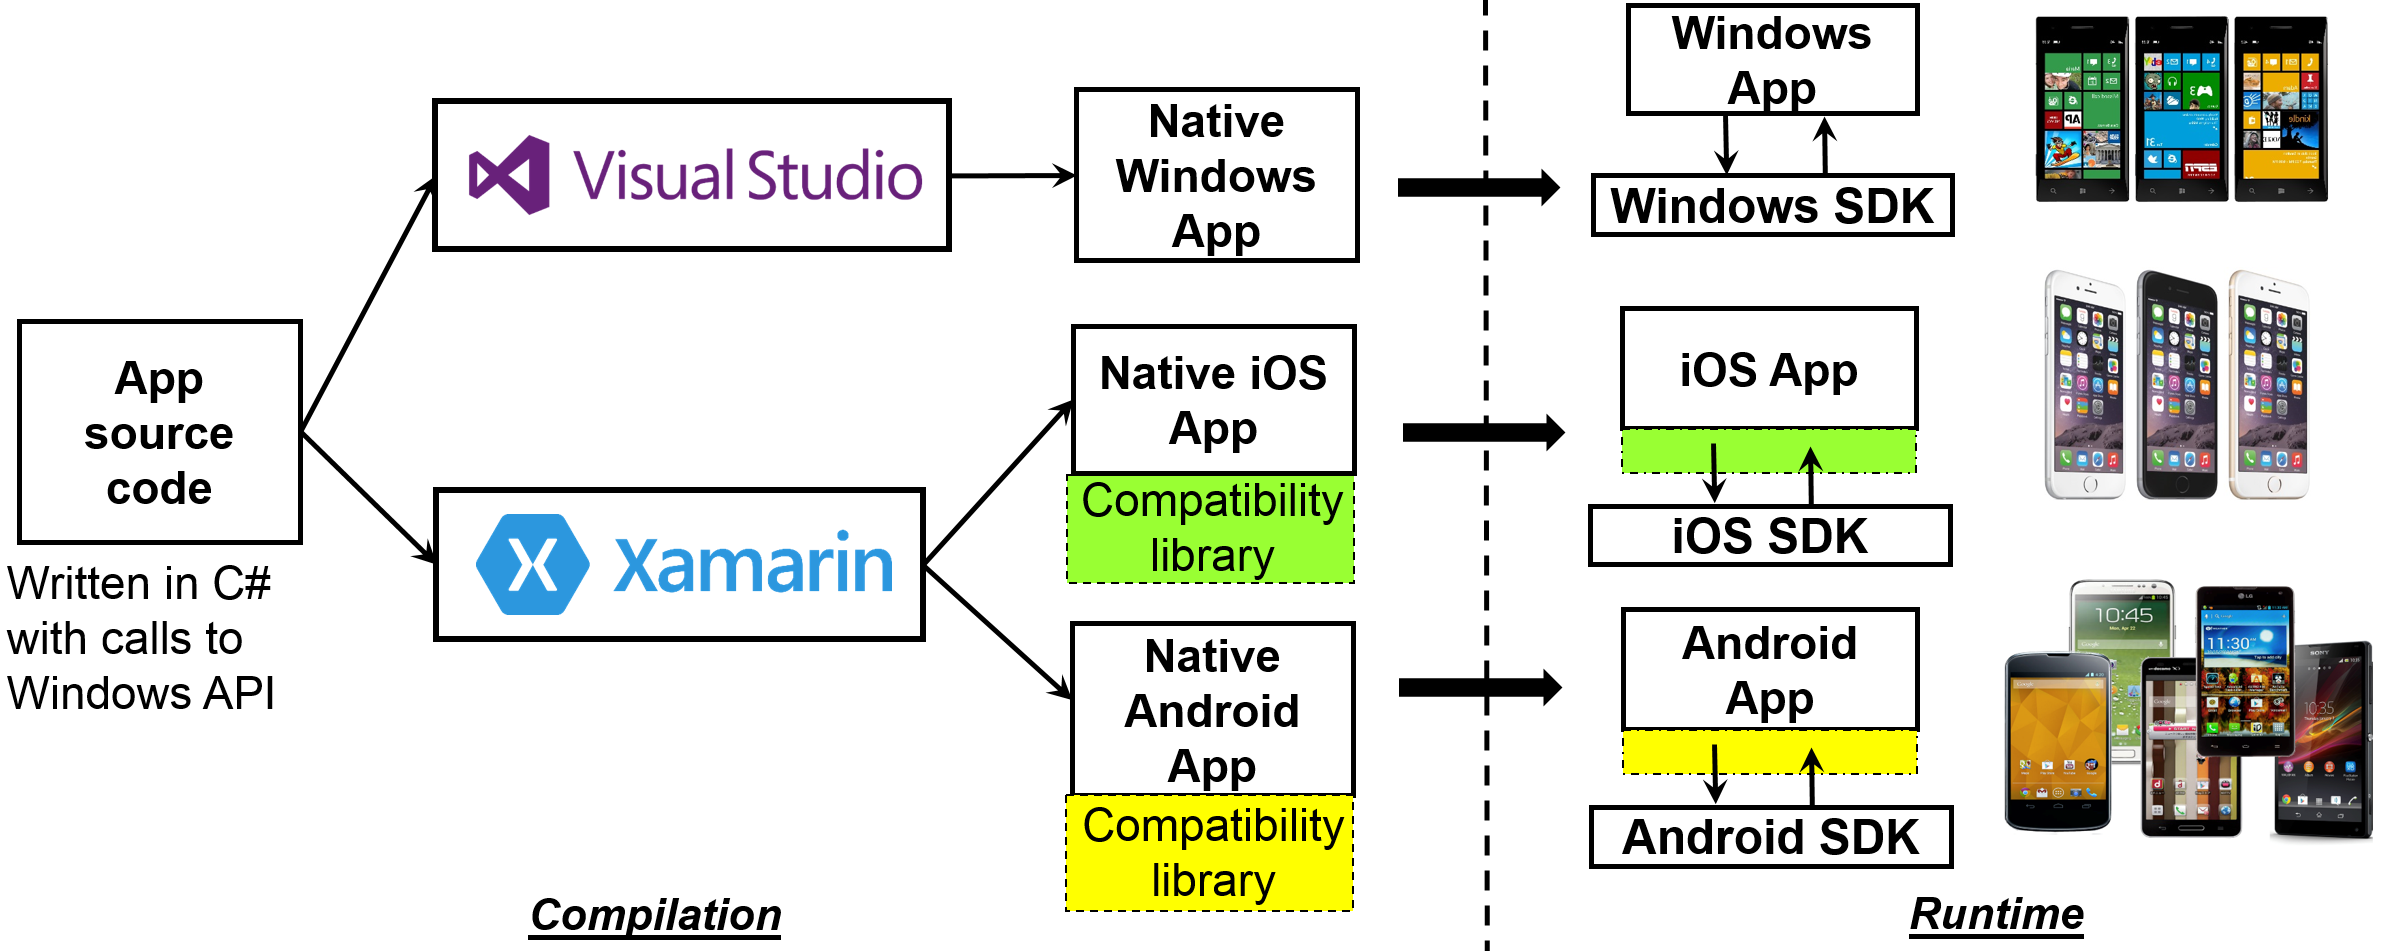
\includegraphics[keepaspectratio=true,width=0.9\textwidth]{figures/xptools-overview.png}
\mycaption{Overall operation of a cross-platform mobile app development
framework, using Xamarin as a concrete example. Developers build apps as they
would for the Windows Phone, in C\# using calls to the API of the Windows Phone
SDK. This code can directly be compiled to Windows Phone apps using the Visual
Studio toolchain. Xamarin allows developers to use the same source code to
build native Android or iOS apps. Xamarin provides compatibility libraries
that translate Windows SDK API calls in the code to the relevant API calls of
the underlying Android and iOS SDKs.}{\label{figure:xplatform-overview}}
\end{figure*}

There are two broad classes of cross-platform frameworks available today.  The
first class, which we call \textit{Web-based frameworks}, allows developers to
build mobile apps using languages popularly used to build Web applications,
such as HTML5, JavaScript, and CSS. Examples of such frameworks include Adobe
PhoneGap~\cite{phonegap}, Sencha~\cite{sencha} and IBM
MobileFirst~\cite{worklight}.  Developers specify the app's logic and user
interface using one or more of the Web-development languages.  However, these
languages do not contain primitives to allow apps to access resources on the
phone, \eg~peripherals such as the camera and microphone, the address book, and
phone settings. Thus, Web-based frameworks provide supporting runtime libraries
that end-users must download and execute on their mobile devices. Mobile apps
interface with these libraries to access resources on the mobile devices---such
mobile apps are also popularly called hybrid mobile apps.  Web-based frameworks
allow developers to rapidly prototype mobile apps.  However, these frameworks
are ill-suited for high-performance apps, such as games or those that use
animation. The expressiveness of the resulting mobile apps is also limited by
the interface exported by the runtime libraries offered by the frameworks.


The second class, which we call \textit{native frameworks}, addresses the above
challenges. Examples of such frameworks include Xamarin~\cite{xamarin},
Apportable~\cite{apportable} and MD$^2$~\cite{md2:sac13,myappconverter}. These
frameworks generally support a \textit{home platform} and one or more
\textit{target platforms}. Developers build mobile apps as they normally would
for the home platform, and leverage the framework's support to automatically
produce apps for the target platforms as well. For example, the home platform
for Xamarin is Windows Phone, and developers build apps using C\# and the API
of the Windows Phone SDK. The Xamarin framework allows developers to
automatically build Android and iOS apps using this code base (see
\figref{figure:xplatform-overview}). Likewise, the home platform for Apportable
is iOS. Developers build apps using Objective-C and the iOS SDK, and leverage
Apportable to produce Android apps from this code base.  In this paper, we will
focus on native frameworks for cross-platform mobile app development. 

When an app developer uses native frameworks, he implicitly expects the apps to
behave consistently across the home and target platforms. Realizing this
expectation depends to a large extent on the fidelity with which the native
framework translates the API calls to SDK of the home platform to the
corresponding SDK of the target platform(s). Unfortunately, this translation is
a complex task because the platform must correctly encode the semantics of both
the home platform and target platform SDK and the relationship between them.
This complexity translates into bugs in the frameworks, \eg~as of mid-December
2014, Xamarin's Bugzilla database shows a history of about 17,600 bug reports,
5,100 of which are still unresolved (listed as ``open'' or ``new''), while
Apportable's bug database shows a history of 820 bug reports, 449 of which are
unresolved.

In this paper, we develop an approach to test native cross-platform app
development tools. Specifically, we aim to discover cases where the behavior of
the application on the home platform is inconsistent with the behavior of its
counterpart on a target platform. Our approach is based on \textit{differential
testing}~\cite{mckeeman:difftest:1998}. We generate random test cases (using
methods described in prior work~\cite{randoop:icse07}), which in our case are
mobile apps in the source language of the home platform. We then use this code
to produce two versions of the app, one for the home platform, and one for the
target platform using the native framework. We then execute the apps and
examine the resulting state for inconsistent behavior.  When two versions of
the app are produced from the same source code, any differences in the behavior
across the versions are indicative of a problem either in the home platform's
SDK, the target platform's SDK, or the way the native framework translates
between the two SDKs.

To realize this approach, we must address two issues::
%
\begin{mylist}
%
\item \textbf{How can we generate effective test cases?} The key research
challenge here is that the space of valid programs that we can generate as test
cases is essentially unbounded. While we could sample from this space, the
effectiveness of these test cases in inducing inconsistent behavior is
questionable.

To address this challenge, we observe that the main difficulty in building
cross-platform mobile app development tools is \textit{translating between the
semantics of the SDKs of the home and target platforms}. Our test-case
generator therefore produces programs that contain random sequences of
invocations to the home platform's SDK. We then observe whether the resulting
apps on the home and target platforms behave consistently. By focusing on the
SDK alone, our approach narrows testing to the most error-prone components of
the cross-platform frameworks.

\item \textbf{How can we check for inconsistent behavior?} Each of our test
cases is compiled into a full-fledged app, one each for the home and target
platforms. When we run the corresponding apps, we must observe their behaviors
to identify inconsistencies. The main research challenge here is in defining a
suitable notion of ``behavior.''

We address this challenge by observing all data structures that are reachable
from the variables defined in the test cases. We serialize these data
structures into a standard format, and compare the serialized versions on the
home and target platforms. Assuming that the state of the home and target
platforms is the same before the test cases are executed, the final state in
each platform after the test cases have been executed must also be the same.
If not, we consider this inconsistent behavior and report an error.
%
\end{mylist}

We have prototyped this approach in a tool called \tool, which we have applied
to test the Xamarin framework using Android as the target platform. Using
\tool, we have found \checkme{47} inconsistencies, which corresponded to bugs
either in Xamarin or the Microsoft SDK (we have reported many of these to
Xamarin or Microsoft). To date, one of these bugs has also been fixed in the
development branch of Xamarin.

\mysection{Restricted Space Usage Model}
\label{section:usagemodel}

We now provide an overview of the restricted space model, motivate some
features of our enforcement mechanism, and describe our threat model.

\subsection{Overall Workflow}

\myparagraph{Check-in}
As depicted in \figref{figure:restrictedspaces}, when a guest enters a
restricted space in which he wishes to use his devices, he ``checks-in'' each
of his devices during entry. During check-in, the guest device communicates
with the host's policy server for the following tasks:

\begin{mylist}
%
\item \textit{Authentication.} The authentication step allows the guest and
host to mutually identify each other. We assume that both the guest and the
host have cryptographic credentials (\eg~public/private key pairs) that can be
validated via a trusted third party, such as a certifying authority. The host
and the guest mutually authenticate each other's credentials in the standard
way, for example, as is typically done during SSL/TLS handshakes.

The host's policies are enforced by a mechanism that executes in the guest.  As
previously discussed, this mechanism is part of the TCB, and must therefore not
be tampered by the guest.  We rely on secure hardware on the guest device (the
ARM TrustZone) to ensure this property.  In particular, we rely on the secure
hardware to detect and prevent any attempts to tamper with the TCB on the
guest. This can be ensured using a special boot-time protocol implemented atop
the secure hardware.

It is important to note that this TCB is \textit{not} the end-user's usual work
environment on the device, \eg~the traditional Android, iOS or Windows
environment with apps. Rather, the TCB is an environment that is created and
distributed by a trusted entity, such as the device vendor, and executes in
isolation on the guest device. 

% NOTE: Clarification from Ferdinand -- this is not how attestation works on
% the TZ as there is no hardware root of trust on the device. Rather vendors
% lock down the secure world and implement secure boot within it.
%
% The host checks the trustworthiness of the TCB by attesting the software
% stack that executes the policy enforcement mechanism.  This attestation is
% typically done from the hardware-up, and is used to ensure that the TCB
% booted correctly and only executes software components that can be trusted by
% the host.  
%
% We can therefore assume that the correct configurations of the TCB are
% well-known to the host, thereby enabling attestation. As we will describe in
% \sectref{section:mechanism}, our TCB on guest devices is simple in its
% functionality and small in size. We attest this TCB using trusted hardware on
% the guest device (the ARM TrustZone) as the root of trust, but other
% implementations may be possible.

\item \textit{Host analyzes device.} The host leverages the TCB to analyze the
guest device. Our mechanism allows hosts to \textit{remotely fetch memory
pages} (and CPU register state) belonging to the guest device.  The TCB
computes a cryptographic checksum over the memory pages to ensure that they are
not tampered with as they are transferred from the guest to the host. 

The host uses raw memory pages from the device in two ways. First, it scans
memory pages to ensure that the device is free of malicious software, \eg~in
the form of malicious apps or kernel modules.  Second, it extracts
configuration information from the device. This includes the kernel version,
the list of peripherals supported by the device, memory addresses of various
device drivers for peripherals on the device and the state of these peripherals
(\eg~whether a certain peripheral is enabled and its settings). The host can
also checkpoint the state of these peripherals so that they can be restored at
check-out. 

\item \textit{Host modifies guest's configuration.} The host modifies the guest
device's configuration to conform to its restricted usage policies.  In the
example shown in \figref{figure:restrictedspaces}, the host's policy is to
disable the camera and the 3G/4G data plan on all devices. The host enforces
this policy by creating a sequence of \textit{remote memory writes} that
directly modify the memory state of the device. For example, the host could
prevent the use of the camera and 3G/4G data plan by unlinking the device
drivers corresponding to the camera and the modem. The host uses the
configuration information extracted in the previous step to determine the
memory addresses that must be modified to unlink these drivers. 

We assume that it is the host's responsibility to ensure that these
configuration modifications are not easily bypassable. For example, these
modifications may be undone if the user of the guest device can directly modify
kernel memory, \eg~by dynamically loading kernel modules or using
\code{/dev/kmem} in the end-user's work environment. The host must use the
inspection phase to identify device configurations that could lead to such
attacks, and disallow the use of such devices in the restricted space.

\item \textit{Host obtains verification token from guest.} After the guest
device has been configured, the TCB produces a \textit{verification token} to
be transmitted to the host. The verification token is an unforgeable value that
encapsulates the set of configuration changes to the device. The TCB computes
the token as a checksum over the memory locations that were modified.  The
token is unforgeable in that only the TCB can re-create its value as long as
the device configuration has not been altered, and any malicious attempts to
modify the token can be detected by the TCB and the host.

At any point when the device is in the restricted space, the host can request
the TCB on the device to send it the verification token. The TCB computes this
token afresh, and transmits it to the host,\footnote{This assumes that the
host's policy still allows a communication channel between the host and the
guest. If all of the guest's peripherals are disabled, the host will need
physical access to the guest to visually obtain the freshly-computed
verification token.} which compares this freshly-computed token with the one
obtained during check-in. It can use this comparison to ensure that the guest
has not altered the device configurations from the previous step.  The
verification token is ephemeral, and can be computed afresh by the guest only
within an expiration period.  In our prototype, the TCB cannot recompute the
verification token if the guest device is rebooted, thereby ensuring that
end-users cannot undo the host's configuration changes by simply rebooting the
device.
%
\end{mylist}

\myparagraph{Check-out}
Once checked-in, the guest device can freely avail of the facilities of the
restricted space under the policies of the host. For example, in
\figref{figure:restrictedspaces}, the smart glass can pair with the smart phone
via Bluetooth, while the smart phone can connect to and use the host's WiFi
access point. When the guest exits the restricted space, he checks-out the
device, accomplishing two goals: 
%
\begin{mylist}
%
\item \textit{Host checks guest state.} The host checks guest device's
configuration by requesting the verification token from the device's TCB to
ensure that the configuration has not been altered. If it finds that the
verification token does not match the value obtained from the device at
check-in, it can detain the device for further inspection, \eg~to determine
whether any data from the restricted environment was exfiltrated.

Note that it is not usually possible to differentiate between mismatches that
happen because of benign reasons, such as a device reboot, or malicious ones,
such as when an end-user intentionally modified the peripheral configurations
required by the host. This is because even malicious modifications can be
masked by simply rebooting the device, and making the mismatch seem benign.
Thus, the host's policy to deal with mismatches depends upon the sensitivity of
the restricted environment. For example, in a federal setting, a detailed
forensic examination of the device may be necessary, the possibility of which
could deter a malicious guest from bypassing the host's policy enforcement. As
previously discussed, hosts can request the verification token from the device
at any time when it is in the restricted space. Hosts can use this feature to
frequently check the verification token and narrow down the timeframe of the
violation.

\item \textit{Restoring guest state.} To restore the state of the device, the
end-user could simply reboot the device. The host only modifies the memory of
the device, and not persistent storage. Rebooting therefore undoes all the
memory modifications performed by the host and boots the device from an
unmodified version of the kernel in persistent storage. Alternatively, the host
can restore the state of the guest device's peripherals from a checkpoint
created at check-in. The main challenge here is to ensure consistency between
the state of a peripheral and the view of the peripheral from the perspective
of user-level apps. For example, when the 3G interface is disabled, an app
loses network connectivity. However, because we only modify memory and do not
actually reset the peripheral, the 3G card may have accumulated packets, which
the app may no longer be able to process when the kernel state is restored.
Mechanisms such as shadow drivers~\cite{shadow:tocs06} can enable such ``hot
swaps'' of kernel state, enabling guest devices to continue without
rebooting.
%
\end{mylist}

% \todo{VG}{A security analysis here? -- No need. Fold in any security
% arguments with the corresponding step in the workflow.}

\subsection{Malicious Hosts} 
\label{section:usagemodel:malicious}
%
Our discussion so far has assumed that hosts are benign. Authentication at
check-in ensures that remote access to guest device memory is available only to
hosts that the guest approves. However, it may be possible even for such hosts
to misuse the facilities of our mechanism to violate the security and privacy
of the guest. For example, a malicious host could use remote memory reads to
obtain the guest's personal data. It could also install a key logger or a
backdoor to spy on the guest's activities. Even if the host is not overtly
malicious, it is possible that the configuration changes that it makes will
render the guest's device vulnerable to attacks. This is reminiscent of the
2006 incident when CD DRM software installed by Sony made the systems on which
it was installed vulnerable to certain kinds of attacks~\cite{sonydrm:sec06}.

To protect guest devices from malicious hosts, we provide a \textit{trusted
vetting service}. We assume that guests register their device(s) with the
vetting service beforehand. When the host sends a remote read/write request,
the guest device forwards the request to the service together with its current
memory configuration. The vetting service analyzes the requests against the
memory configuration and determines whether the request conforms to certain
safety policies. \sectref{section:vetting} presents the details of our vetting
service.

The vetting service could directly be implemented in the TCB executing on the
guest device, but this has the undesirable effect of bloating the TCB on the
device. We therefore implement vetting as a cloud service.  Note that vetting
is optional. If the guest trusts the host, it could carry out the host's
requests without vetting.

% It is challenging to protect guest devices from malicious hosts, and
% \textit{for this paper, we will assume that hosts are benign}. Nevertheless,
% there are a few defenses that could be used to protect against malicious
% hosts.  To protect personal data, privacy-conscious users could store their
% data encrypted on disk and in memory, except when it is used. However, this
% would require apps on the device to be redesigned to be aware of such
% encrypted data.

% To protect against remote writes that maliciously modify the guest device
% (\eg~by installing a keylogger), the guest could rely on a trusted third
% party to vet the operations of the host. That is, the guest could forward its
% memory configuration and the remote operations requested by the host to the
% trusted third party prior to making any memory modifications. The guest would
% proceed with the modifications only if the trusted third party certifies that
% the operations do not install malicious software on the guest device.
% Alternatively, a simpler solution is to restrict the kinds of remote write
% operations that a host can initiate. For example, the TCB could enforce that
% the only remote memory writes available to the host are writing \textsc{null}
% bytes to memory locations that store device driver hooks. This would allow
% hosts to unlink drivers and disable peripherals, but prevent them from
% installing malicious software.

\subsection{Covert Use and Legacy Devices}
%
It is certainly possible for a guest to bypass the host's policies by not
declaring a device during check-in, and using it covertly within the restricted
space. As long as the guest carefully configures the device to avoid accessing
any of the host's resources in the restricted space, \eg~its WiFi access
points, and remain stealthy, the device cannot be detected by the host.

Our focus in this paper is to address policy enforcement for overt uses of
smart devices. Covert uses, such as the above, are out of the scope of the
mechanisms developed in this paper. Instead, we assume that traditional methods
such as physical security checks are necessary to detect covertly-hidden
devices.

Finally, what if the guest uses a ``legacy'' device, \ie~one that is not
equipped with trusted hardware, such as the ARM TrustZone? In
\sectref{section:discussion}, we present a number of design alternatives to
enforce policies on such legacy devices.  However, because they do not use
secure hardware, these alternatives cannot offer the same security guarantees
as our approach, or require larger TCBs on guest devices to offer similar
guarantees. Our take on the issue of legacy device support is that while legacy
devices are certainly important in today's settings, we are beginning to see an
increasing deployment of devices equipped with trusted hardware
(\eg~see~\cite{knox:ccs14}). We hypothesize that moving forward, hosts will
have to contend with fewer legacy guest devices than they do today.

\subsection{Threat Model} 
\label{section:threat}
%
Given the discussion in this section, we now summarize our threat model. 
Each guest device is assumed to be partitioned into two parts: (1)~the
end-user's work environment, and (2)~the environment that runs the policy
enforcement mechanism. 

From the perspective of the host, the end-user's work environment is untrusted.
The host must trust the policy enforcement mechanism, but because it executes
on the guest device, the host leverages secure hardware, the ARM TrustZone in
our case, to bootstrap this trust. Having established trust, the host then uses
the policy enforcement mechanism to securely read and modify the memory state
of the work environment. It is the host's responsibility to inspect the memory
state of the work environment to determine whether it is malicious, contains
known exploitable vulnerabilities, or allows guests to bypass the configuration
changes that the host may make.  Once the host determines that the guest's work
environment is acceptable, it can induce changes to the guest's memory state.
Guests are assumed to keep their devices powered on for the duration of their
stay in the restricted space, failing which the verification tokens will no
longer match. Mismatches may also happen if the guest maliciously modifies the
host's changes.

The work environment may contain zero-day vulnerabilities, such as a
newly-discovered buffer overflow in the kernel. The host may not be aware of
this vulnerability, but a malicious guest may know of it and have an exploit to
bypass the host's policies.  Such threats are outside the scope of our work,
but the host may protect itself by requiring the guest's work environment to
run a fortified software stack (\eg~Samsung Knox~\cite{knox:ccs14} or
MOCFI~\cite{mocfi:ndss12}). The host can check this requirement during the
inspection phase. A malicious work environment may also launch a
denial-of-service attack, which will prevent the host from communicating with
the TCB on the guest device.  However, such attacks can readily be detected by
the host, which can then prevent the device from entering the restricted space.
We exclude such attacks from our threat model.

From the perspective of the guest, if the host is untrusted, it can rely on a
trusted vetting service to determine if the host's read and write requests are
safe.

% the host is assumed to only make benign changes to the guest work
% environment.  However, it may be possible to relax this assumption provided
% the guest vets all the host's intended changes with a trusted third party.
% Similarly, although the host is assumed not to maliciously compromise the
% guest's privacy, a guest may choose to encrypt its in-memory and on-disk data
% to protect it from the host.


% What if kernel module is loaded dynamically? We disable that.




\mysection{Remote Memory Operations}
\label{section:policy}

We now discuss how hosts can use remote memory read and write operations to
analyze and control guest devices.

\myparagraph{Analysis of Guest Devices}
%
A host can analyze memory snapshots of a guest's normal world kernel to
determine its configuration and scan it for kernel malware (also called
kernel-level \textit{rootkits}).

\begin{mylist}
%
\item \emphitem{Retrieving configuration information.} The host can determine the
kernel version by inspecting code pages, thereby also allowing it to check if
the guest has applied recommended security patches. The host can compare a hash
of each kernel code page against a whitelist, \eg~of code pages in approved
Android distributions, to ensure that the normal world is free of malicious
kernel code~\cite{patagonix:sec08,secvisor:sosp07}. Additionally, the host can
ensure that the kernel is configured to disallow well-known attack surfaces,
\eg~access to \textsf{/dev/kmem} and dynamic module loading. Finally, the host
can identify addresses at which functions of a peripheral's driver are loaded,
where they are hooked into the kernel and the addresses that store
memory-mapped peripheral settings. To do so, it can use the recursive memory
snapshot traversal technique described below. The host can use this information
to design the set of memory updates that reconfigure the device to make it
policy-compliant.
%
\item \emphitem{Detecting malicious data modifications.} Rootkits can achieve
malicious goals by modifying key kernel data
structures~\cite{sbcfi:ccs07,shadows:oakland07,specmon:usenix06}.  The attack
surface exposed by kernel data structures is vast.  For instance, a rootkit
could inject a device driver in kernel memory and modify kernel function
pointers to invoke methods from this driver.  Other examples of data structures
that can be misused include process lists, entropy pools used by the kernel's
random number generator, and access control
structures~\cite{shadows:oakland07,specmon:usenix06}.  
%
\end{mylist}

We now describe a generic approach, developed in prior
work~\cite{sbcfi:ccs07,gib:tdsc11,kop:ccs09,kop:sec12,osck:asplos11}, that
hosts can use to detect such malicious data modifications by analyzing the
normal world's memory snapshot. The main idea is to recursively traverse the
memory snapshot and reconstruct a view of the kernel's data structures, and use
this view to reason about the integrity of kernel data. We assume that the host
has access to the type declarations of the data structures used by the guest
device's normal world kernel, \eg~the sizes, layouts, and fields of every data
structure. The host obtains this information from trusted repositories using
the kernel version, extracted as discussed earlier.

Snapshot traversal starts from well-known entrypoints into the system's memory,
\eg~the addresses of the entities in \textsf{System.map}. When the traversal
process encounters a pointer, it fetches the memory object referenced by the
pointer and recurses until all objects have been fetched.  Having reconstructed
a view of kernel data structures, the host can then determine whether they have
been maliciously modified. For example, it could check that function pointers
in the kernel point to functions defined in the kernel's code
space~\cite{sbcfi:ccs07}. Similarly, the host can check that the kernel's data
structures satisfy invariants that typically hold in an uncompromised
kernel~\cite{gib:tdsc11}. We do not further elaborate on specific rootkit
detection policies because they are orthogonal to our focus.

A rootkit-infected OS kernel can be reliably diagnosed \textit{only by
externally observing its code and data}, \eg~using memory snapshots as already
discussed. Prior techniques that enforce policies on guest devices using
security-enhanced, policy-enforcing normal world kernels
(\eg~\cite{asm:sec14,flaskdroid:sec13,conxsense:asiaccs14,worlddriven:ccs14,blindspot:2009,markit:upside14,knox:mdm,ms:intune,blackberry:emm})
can also benefit from our approach to establish normal world kernel integrity
to hosts.

We have restricted our discussion to an analysis of the normal world's kernel
memory snapshot. In theory, it is possible for a host to also request and
analyze the normal world's user-space memory, \eg~for malicious apps that
reside in memory or on the file system. However, in practice, user-space
memory may contain sensitive information stored in apps, which guests may be
unwilling to share with hosts. For example, guests can configure their vetting
service to mark as \textsc{Unsafe} host requests to fetch user-space memory
pages (see \sectref{section:vetting}). 

To ensure user-space security, hosts can leverage the normal world kernel after
establishing that it is benign, \eg~using the snapshot traversal methods
described above. The host can require the normal world kernel to execute a
mutually-agreed-upon anti-malware app in user-space. At check-in, the host
scans the process list in the device's kernel memory snapshot to ensure that an
anti-malware is executing. This app can check user-space memory and the
file-system for malicious activity. At check-out, it can ensure that the same
app is still executing by comparing its process identifier to the value
obtained at check-in,\footnote{The security of this scheme is based on the fact
that PIDs on UNIX systems are, for all practical purposes, unique on a given
system. For example, while they can be recycled, it requires a large counter to
wrap around.} thereby ensuring that the anti-malware app was active for the
duration of the guest's stay.

\myparagraph{Control over Guest Device Peripherals}
%
Hosts can control the availability and configuration of peripherals on guest
devices via remote memory updates to the devices. After analyzing the guest's
memory snapshot, hosts prepare a set of memory updates to control various
peripherals on guest devices. These updates can be used to simply uninstall
peripherals that may be misused violate the host's policies. Our overall
approach to controlling peripherals is to update peripheral device drivers. On
modern OSes, each peripheral has an interface within the kernel. This interface
consists of a set of function pointers that are normally set to point to the
corresponding functions within the peripheral's device driver, which
communicates with the peripheral. 

\begin{figure}[t!]
\begin{center}
\footnotesize
\begin{tabular}{|cc|}
\hline
\multicolumn{2}{|c|}{\indent\vspace{-0.3cm}}\\
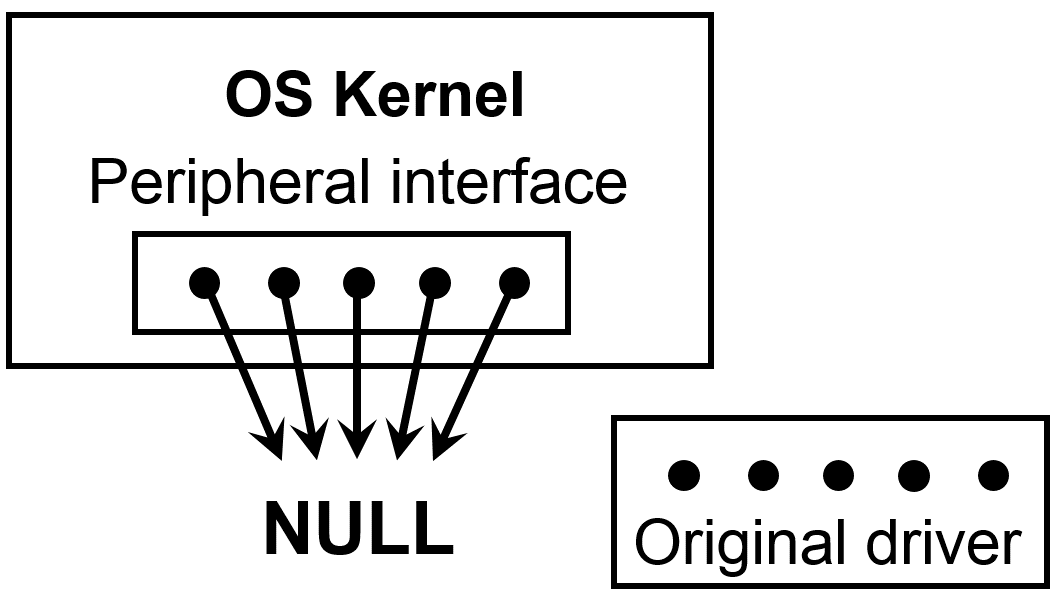
\includegraphics[keepaspectratio=true,height=0.85in]{figures/driver-null.png} & 
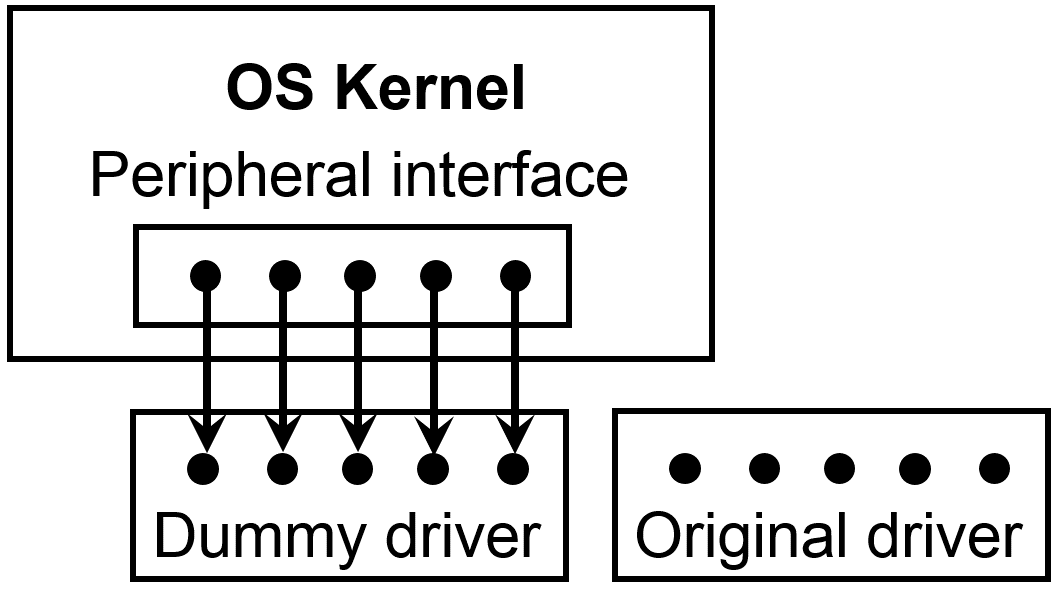
\includegraphics[keepaspectratio=true,height=0.85in]{figures/driver-dummy.png}\\
\textbf{(a)~\textsc{null}ifying the interface} &
\textbf{(b)~Installing a dummy driver}\\
%\indent\vspace{-0.9cm}
\multicolumn{2}{|p{0.47\textwidth}|}
{\small Each device driver exposes an interface and is linked to the kernel via
function pointers.  Part~(a) shows how to uninstall the peripheral by making
the kernel's device interface point to \textsc{null} bytes.  Part~(b) shows how
to uninstall the peripheral by unlinking the original driver and instead
linking a dummy driver.}\\
\hline
\end{tabular}
\end{center}
\indent\vspace{-0.5cm}
\mycaption{Uninstalling peripheral device drivers using remote write operations 
to kernel memory.}
{\label{figure:uninstall}}
\end{figure}

We adopted two broad strategies to update device drivers:  

\begin{mylist} 
%
\item \emphitem{Nullifying interfaces (\figref{figure:uninstall}(a)).} This
approach simply sets the function pointers in the peripheral's interface to
\textsc{null}. If the kernel checks these pointers prior to invoking the
functions, it will simply return an error code to the application saying that
the device is not installed. This approach has the advantage of only involving
simple writes to the kernel (\textsc{null} bytes to certain addresses), which
can easily be validated as safe if the guest so wishes. However, we found in
our evaluation (\sectref{section:evaluation}) that this approach can crash the
device if the kernel expects non-\textsc{null} pointers.
%
\item \emphitem{Dummy drivers (\figref{figure:uninstall}(b)).} In this approach,
the host writes a dummy driver for the peripheral and links it with the kernel
in place of the original driver. If the dummy driver simply return a suitable
error code rather than communicating with the peripheral, it has the effect of
uninstalling the peripheral. The error code is usually bubbled up to and
handled by user apps. Some apps may not be programmed to handle such errors, so
an alternative approach could be for the dummy driver to return synthetic
peripheral data instead of error codes~\cite{mockdroid:hotmobile10}. Dummy
drivers can also offer fine-grained peripheral control. For example, with
3G/4G, it may be undesirable to simply uninstall the modem to disable voice
messaging because it also prevents the guest from making emergency calls. The
host can avoid this by designing a dummy driver that allows calls to emergency
numbers alone, while disabling others. In this approach, the host introduces
new driver code into the guest. From the guest's perspective, this code is
untrusted and must be safety-checked by the vetting service.

\end{mylist}


\mysection{Policy Enforcement}
\label{section:mechanism}

We now present the design of our policy enforcement mechanism. Although the
core of our mechanism that relies on remote memory operations is platform
agnostic, we describe it in the context of the ARM TrustZone. We leverage the
TrustZone's features to isolate the enforcement mechanism and to bootstrap its
security features. We present alternative designs in
\sectref{section:discussion:alternatives}.

\subsection{Background on ARM TrustZone}
\label{section:mechanism:armback}

The TrustZone is a set of security enhancements to chipsets based on the ARM
architecture. These enhancements cover the processor, memory and peripherals.
With TrustZone, the processor can execute instructions in one of two security
modes at any given time, a \textit{normal world} and a \textit{secure world}. A
third \textit{monitor mode} facilitates switching between the normal and the
secure worlds.  The secure and normal worlds have their own address spaces and
different privileges.  The processor can switch from the normal world to the
secure world via an instruction called the secure monitor call (\texttt{smc}).
When an \texttt{smc} instruction is invoked from the normal world, the
processor context switches to the secure world (via monitor mode) and freezes
execution of the normal world.

TrustZone can partition memory into two portions, with one portion being
exclusively reserved for the secure world. It also allows individual
peripherals to be assigned to the secure world.  For these peripherals,
hardware interrupts are directly routed to and handled by the secure world.
While the normal world cannot access peripherals or memory assigned to the
secure world, the secure world enjoys unrestricted access to all memory and
peripherals on the device. It can therefore access the code and data 
of the normal world. The secure world can execute arbitrary software,
ranging from simple applications to an entire operating system.
%
% NOT the CPU state. Registers are "banked", and only monitor mode can view
% them all.

A device with ARM TrustZone boots up in the secure world. After the secure
world has initialized, it switches to the normal world and boots the operating
system there. Most TrustZone-enabled devices are configured to execute a
\textit{secure boot} sequence that incorporates cryptographic checks into the
secure world boot process~\cite{armtz}. For example, the device vendor could
sign the code with its private key, and the vendor's code in the boot ROM would
verify this signature using the vendor's public key. These checks ensure that
the integrity of the boot-time code in the secure world has not been
compromised, \eg~by reflashing the image on persistent storage. Most vendors
lock down the secure world via secure boot, thereby ensuring that it cannot be
modified by end-users. This feature allows hosts to trust software executing in
the secure world and treat it as part of the TCB. In the rest of this paper, we
will assume that our guest devices use the secure boot process.

\subsection{Overall Design}
\label{section:mechanism:overall}

\begin{figure}[t!]
\centering
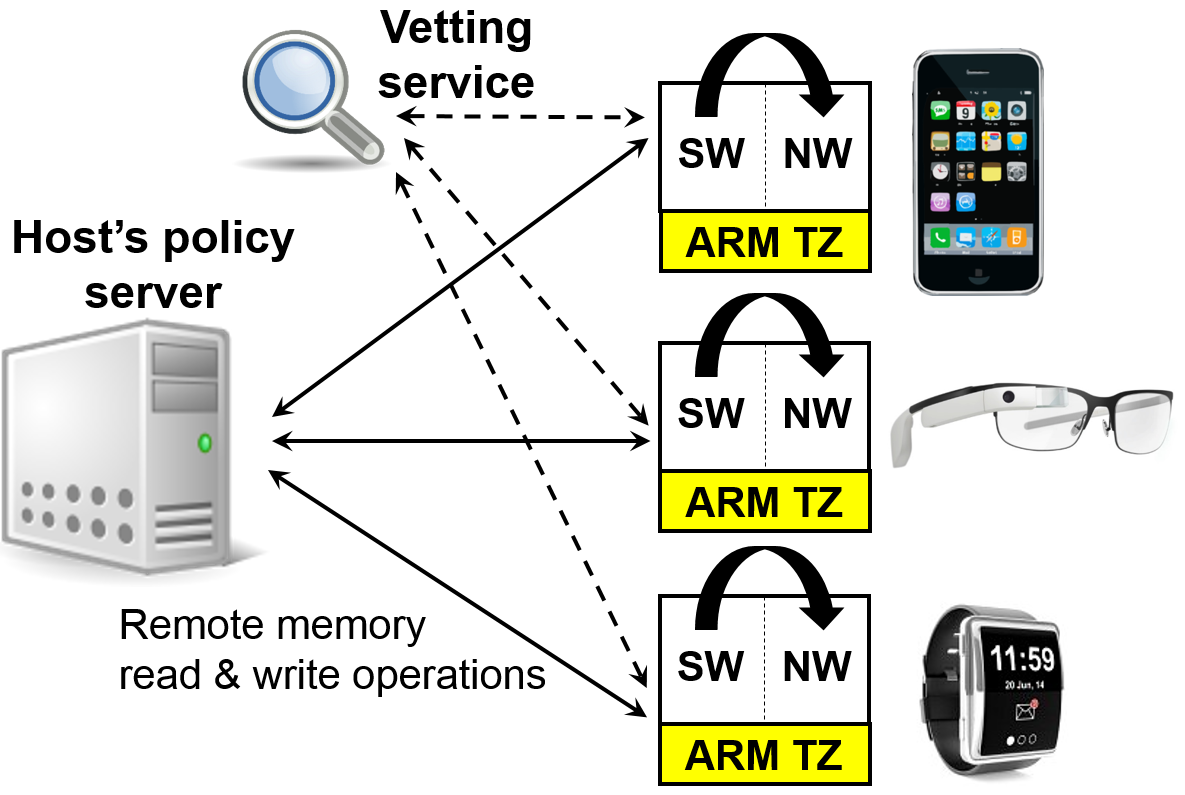
\includegraphics[keepaspectratio=true,width=0.45\textwidth]{figures/host-guest.png}
%\indent\vspace{-0.2cm}
\mycaption{Overall setup showing communication between the host and guest
devices. Guest devices are equipped with ARM TrustZone and execute components
of the policy enforcement mechanism (see \figref{figure:overall}).  Abstractly,
the goal is to establish a communication channel between the host's policy
server and the enforcement mechanism running in the secure world (SW) of the
guest devices. The host leverages the secure world to remotely inspect and
modify normal world (NW) memory.}
{\label{figure:hostguest}}
%\indent\vspace{-0.3cm}
\end{figure}


\figref{figure:hostguest} shows the overall setup of our framework. The host
runs a policy server that communicates with guest devices in its restricted
space. The normal world of each guest executes the end-user's work environment,
and can run a full-fledged mobile operating system---in our prototype the
normal world executes Android. Because this code is under the control of the
end-user, the normal world is untrusted. The secure world of the guest runs a
TCB that accepts and processes the operations remotely-initiated by the host to
inspect the guest device and regulate the use of its peripherals. 

For this setup to work, we need a communication channel that allows the host to
securely relay its requests to the guest and obtain the guest's responses. In
particular, the channel must not allow an attacker, such as the untrusted code
executing in the normal world, to tamper with messages transmitted on it.

One way to set up such a channel is to configure the secure world to directly
communicate with the host. In this case, the secure world would exclusively
control a communications peripheral, say WiFi, and establish a connection with
the host without involving the normal world. Thus, the code necessary to
support this peripheral must also execute within the secure world and be part
of the TCB. With WiFi, for instance, this would mean that several thousand
lines from the networking stack would need to execute within the TCB.

In our work, we chose an alternative approach that minimizes the functionality
implemented in the TCB. In this approach, the normal world mediates the
communication channel between the secure world and the host, and is assigned
all the peripherals on the device. Because the normal world is untrusted, the
secure world and the host include cryptographic checksums with each message
transmitted on the channel, and sanity-check the messages before processing
them. The secure world itself executes a bare-minimum TCB that performs just
three key operations:
%
(1)~mutual authentication (\sectref{section:mechanism:auth}), 
%
(2)~remote memory operations (\sectref{section:mechanism:rmo}),
%
(3)~verification tokens (\sectref{section:mechanism:tokens}). 

\begin{figure}[t!]
\centering
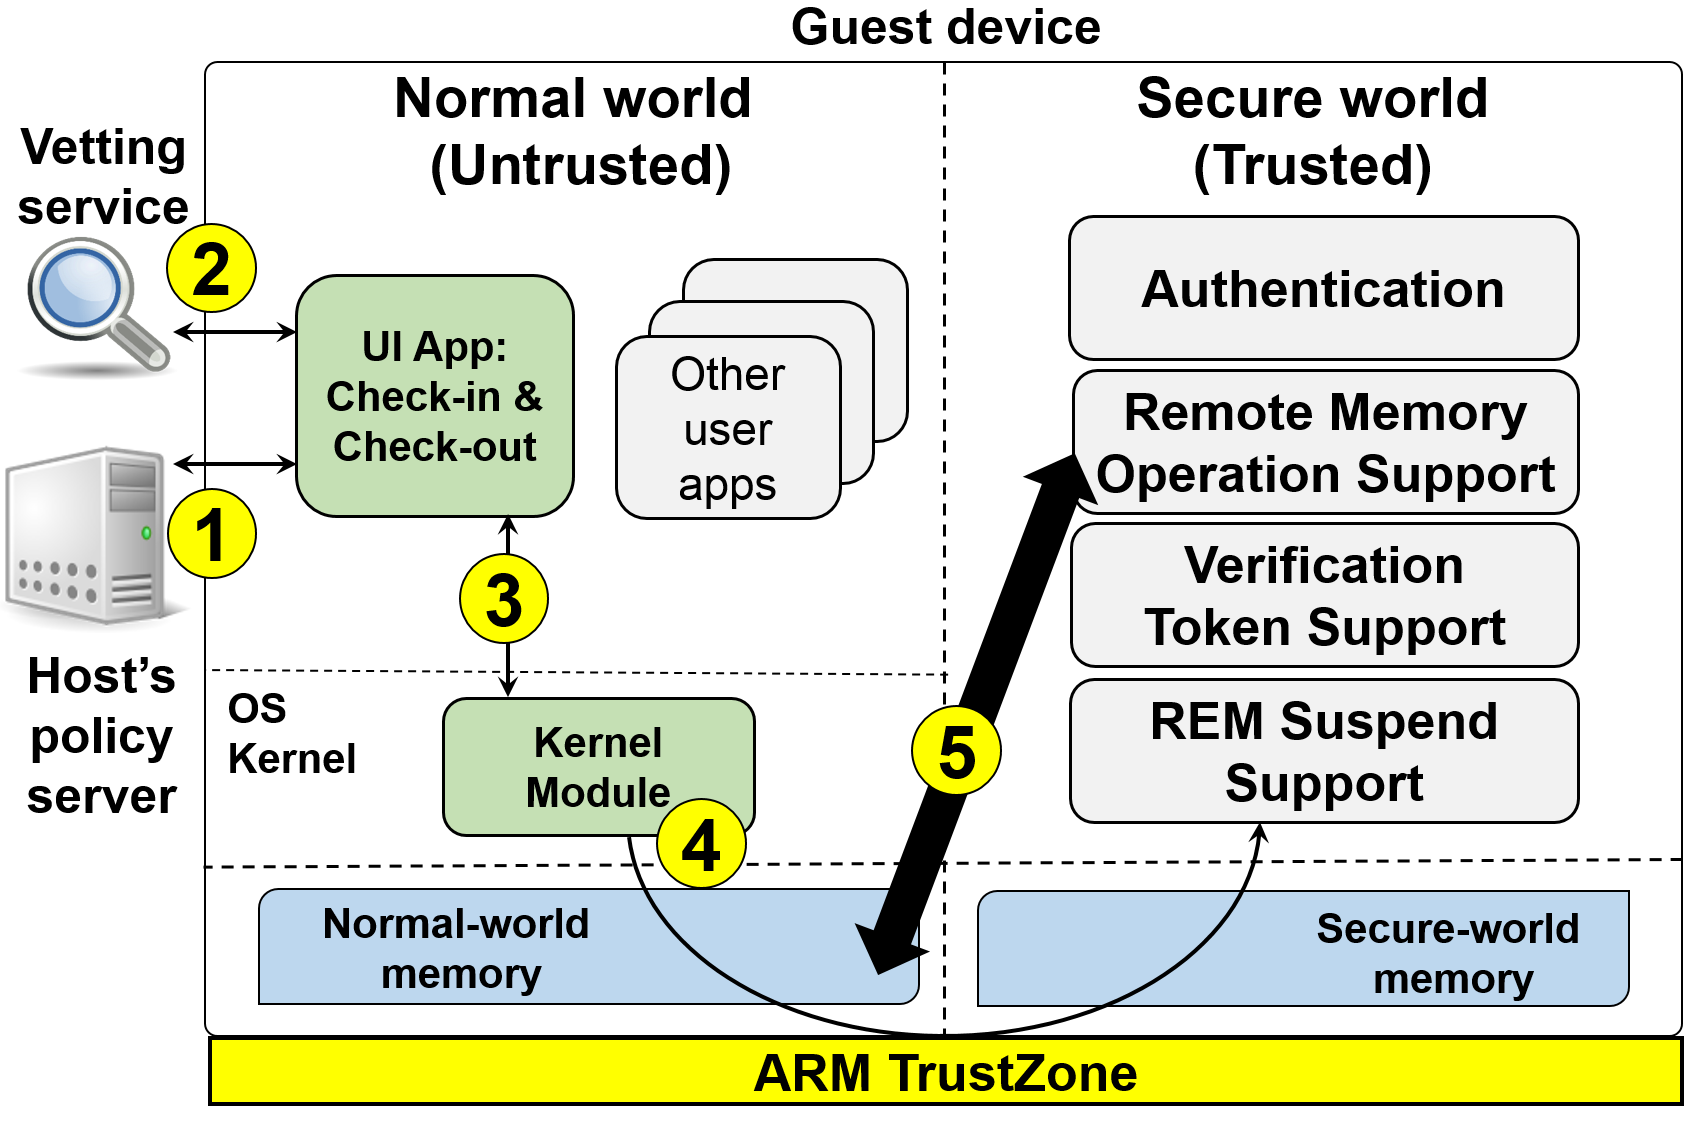
\includegraphics[keepaspectratio=true,width=0.45\textwidth]{figures/overall-design.png}
%\indent\vspace{-0.1cm}
\mycaption{Guest device setup showing components of the policy enforcement
mechanism. (1)~The host communicates with the UI app on the guest and sends
requests to perform remote memory operations. (2)~The UI app uses the vetting
service to determine the safety of the request. (3)~If determined to be safe,
the UI app forwards this request to the supporting kernel module. (4)~The
kernel module invokes the secure world by performing a world switch. (5)~The
secure world performs the requested memory operations on the normal world
memory on behalf of the host.  The components in the normal world, \ie~the UI
app and the kernel module are untrusted. The TCB consists of only the
components that execute in the secure world.}{\label{figure:overall}}
%\indent\vspace{-0.3cm}
\end{figure}

Guest devices are therefore set up as shown in \figref{figure:overall}.  Within
the normal world, the end-user interacts with the host as well as with the
secure world via a user-level app (called the UI app).  This app serves as the
end-user's interface to the host, allowing him to perform operations such as
check-in and check-out of the device. The app interacts with the components in
the secure world via a kernel module. The host sends a request to perform
remote memory operations on the guest device to the app. The app determines the
safety of this request using the vetting service (\sectref{section:vetting}),
and forwards the request to the kernel module, which invokes \texttt{smc} to
world switch into secure world. The components of the secure world then perform
the request and communicate any return values to the host via the UI app. 

We do not place any restrictions on how the host communicates with the guest.
Thus, the host's policy server could be hosted on the cloud and communicate
with the guest device over WiFi or 3G. Alternatively, the host could install
physical scanners at a kiosk or on the entryway to the restricted space.  The
guest devices would use Bluetooth, NFC, or their USB interface to pair with the
scanner and use it to communicate with the host.

One of the key features of our approach is that the core mechanisms that run
on the TCB in the guest device are \textit{platform-agnostic} and
\textit{policy-agnostic}.  Rather, they present a narrow read/write interface
that hosts can suitably use to enforce policy. All the complex tasks of device
analysis and deciding policy are shifted to the host. Thus, in principle, we
can use the same TCB mechanisms on guest devices that run Android, iOS and
Windows. Hosts would have separate modules to analyze and control each kind of
guest platform.

\subsection{Authentication}
\label{section:mechanism:auth}
\newcommand{\ks}{$k_s$}
\newcommand{\pub}[1]{{\sf Pub#1}}
\newcommand{\prv}[1]{{\sf Prv#1}}
\newcommand{\enc}[2]{\textsf{Enc}$_{#1}$(#2)}
\newcommand{\cert}[1]{\textsf{Cert}(#1)}

Before accepting any remote memory requests, the guest and the host mutually
authenticate each other. We assume that both the host and the guest device have
public/private key pairs with digital certificates issued by a certifying
authority. The guest device stores its private key \prv{G} in its secure world,
thereby protecting it from the untrusted normal world. 

\begin{figure}[t!]
\footnotesize
\centering
\begin{tabular}{|rll|}
\hline
\multicolumn{3}{|l|}{Let host's public/private keypair be \pub{H},~\prv{H}.}\\
\multicolumn{3}{|l|}{Let guest's public/private keypair be \pub{G},~\prv{G}.}\\
1. & \textbf{Guest} $\rightarrow$ \textbf{Host}:
   & \pub{G}, \cert{\pub{G}}\\
%
2. & \textbf{Host} $\rightarrow$ \textbf{Guest}:
   & \pub{H}, \cert{\pub{H}}\\
%
3. & \multicolumn{2}{p{0.42\textwidth}|}{Guest and host verify
       \cert{\pub{H}} and \cert{\pub{G}}}\\
%
4. & \textbf{Host} $\rightarrow$ \textbf{Guest}:
   & $M$, \enc{\prv{H}}{$M$} (\ie~host signs $M$),\\
%
   & \multicolumn{2}{p{0.42\textwidth}|}{where $M$ is 
	      \enc{\pub{G}}{\ks, timestamp}}\\
%
5. & \multicolumn{2}{p{0.42\textwidth}|}{Guest verifies host's digital 
        signature, decrypts M to obtain \ks, and checks timestamp}\\
%
\hline
\end{tabular}
%\indent\vspace{-0.3cm}
\mycaption{Mutual authentication and establishment of \ks.}
{\label{figure:authentication}}
%\indent\vspace{-0.3cm}
\end{figure}

Authentication is akin to TLS handshakes (\figref{figure:authentication}). The
host and the guest exchange public keys and validate the certificates of these
keys with the issuing authority. The host then computes a session key \ks,
which is then transmitted to the client over an secure channel. Note that \ks\
is only used to protect the integrity of messages transmitted between the guest
and the host and not its secrecy.  The key \ks\ is stored in secure world
memory, and is invisible to the normal world. If the guest is rebooted, \ks\ is
erased from memory.

\subsection{Remote Memory Operations}
\label{section:mechanism:rmo}

\myparagraph{Remote Reads} 
%
The host inspects and modifies the guest device's configuration via remote
memory operations. During check-in the host typically requests the guest to
send raw memory pages from the normal world for analysis.  The UI app receives
this request and performs a world switch to complete the request.  The world
switch suspends the UI app and transfers control to the secure world.  Each
request is a set of virtual memory addresses of pages that must be sent to the
host.   The host also includes a message-authentication code (a SHA1-based HMAC
in our case) with the request. The HMAC is over the body of the request using
the key \ks\ negotiated during the authentication phase.

The secure world checks the integrity of the request using the HMAC. This step
is necessary to ensure that the request was not maliciously modified by the
untrusted components in the normal world. The secure world then translates each
virtual page address in the request to a physical page address by consulting
the page table in the normal world kernel. In this case, the page table will
correspond to the suspended context in the normal world, \ie~that of the UI
app, into which the running kernel is also mapped.  It then creates a
local copy of the contents of this physical page from the normal world, and
computes an HMAC over the page (again using \ks). The page and its HMAC are
then copied to a buffer in the normal world, from where they can be transmitted
to the host by the UI app.  The host checks the HMAC and uses the page for
analysis. This process is iterative, with the host requesting more pages from
the guest based upon the results of the analysis.

Note that in our case, both the host and the secure world are isolated from the
normal world, which is untrusted. We only rely on the normal world kernel to
facilitate communication between the host and the secure world. Moreover, both
the host and the secure world use HMACs to protect the integrity of messages
transmitted via the normal world.  The normal world may drop messages and cause
a denial-of-service attack; however, such attacks are outside our threat model
(see \sectref{section:threat}). The host can therefore reliably obtain the
memory pages of the normal world to enable the kinds of analyses described in
\sectref{section:policy:analysis}. Communication between the host and the
secure world is not confidential and is therefore not encrypted.\footnote{The
host and guest could communicate over TLS, but the TLS channel on the guest
ends at the UI app, which runs in the normal world.} Thus, a malicious normal
world kernel can potentially snoop on the requests from the host to fetch pages
and attempt to remove the infection to avoid detection. However, this would
have the desirable side-effect of cleaning the guest device at check-in.

\myparagraph{Remote Writes}
%
The host reconfigures the guest by modifying the running state of the normal
world kernel via remote write requests. Each write request is a set of triples
$\langle$\textit{vaddr}$_i$,~\textit{val}$_i$,~\textit{old-val}$_i$$\rangle$
together with an HMAC of this request. The normal world conveys this request to
the secure world, which verifies the integrity of the message using its HMAC.
For each virtual address \textit{vaddr}$_i$ (which refers to a memory location
in the virtual address space of the UI app) in the request, the secure world
ensures that the current value at the address matches \textit{old-val}$_i$.  If
all the values match, then the secure world replaces their values with
\textit{val}$_i$. 

Note that because the normal world is frozen during the course of this
operation, the entire update is atomic with respect to the normal world. When
a remote write operation succeeds, the secure world computes and returns a
verification token to the host. If not, it returns an error code denoting a
failure.

A remote write request can fail if the value stored at the virtual address
\textit{vaddr}$_i$ does not match the value \textit{old-val}$_i$.  This problem
arises in our design because the host's remote read and write operations do not
happen as an atomic unit. The host remotely reads pages copied from the normal
world's memory, analyzes them and creates remote write request using this
analysis. During this time, the normal world kernel continues to execute, and
may have updated the value at the address \textit{vaddr}$_i$.

If a remote write operation fails, the host repeats the operation until it
succeeds. That is, it refetches pages from the guest, analyzes them, and
creates a fresh write request. In theory, it is possible that the host's write
requests will fail \textit{ad infinitum}. However, for the setting that we
consider, write operation failures are rare in practice. This is because our
write operations modify the addresses of peripheral device driver hooks.
Operating systems typically do not change the values of device driver hooks
after they have been initialized at system boot. 

In theory, a remote write request can also fail if the virtual address
\textit{vaddr}$_i$ referenced in the request is not mapped to a physical page
in memory, \ie~if the corresponding page has been swapped out to persistent
storage. In practice, however, we restrict remote writes to kernel data pages
that are resident in physical memory, as is the case with device drivers and
pages that store data structures of peripherals. Therefore, we do not observe
failures due to a failure to resolve \textit{vaddr}$_i$s.

It is possible to completely avoid such problems by design if we complete both
the read and write operations in a single world switch. During this time, the
normal world remains frozen and cannot change the view of memory exported to
the host.  The read and write operations will therefore happen as an atomic
unit from the normal world's perspective. However, in this case, the secure
world must have the ability to directly communicate with the host. As already
discussed in \sectref{section:mechanism:overall}, we decided against this
design because it has the unfortunate consequence of bloating the size of the
TCB.  Thus, we make the practical design tradeoff of minimizing the
functionality of the TCB while allowing the rare remote write failure to
happen.

\subsection{Verification Tokens}
\label{section:mechanism:tokens}

The host receives a verification token from the secure world upon successful
completion of a remote write operation. A verification token \textsf{VTok}[$r$]
is the value
%
%\begin{center}
%
$
r||\textit{MemState}||\textsf{HMAC}_{k_s}[r||\textit{MemState}]$
%
%\end{center}
%
where \textit{MemState} is
$\langle\textit{vaddr}_1,~\textit{val}_1\rangle||\ldots||\langle\textit{vaddr}_n,~\textit{val}_n\rangle$,
the set of \textit{vaddr}$_i$ modified by the remote write, and the new values
\textit{val}$_i$ at these locations. The token \textsf{VTok}[$r$] is
parameterized by a random nonce $r$. This nonce can either be provided by the
host together with the remote write request, or can be generated by the secure
world. 

Verification tokens allow the host to determine whether the guest attempted to
revert the configuration changes made by the remote write, either maliciously
or by turning off the guest device. To do so, the host obtains a verification
token \textsf{VTok}[$r_{{\it checkin}}$] upon completion of checkin, and
stores this token for validation. During checkout, the host requests a
validation token \textsf{VTok}[$r_{\it checkout}$] from the guest over the
same virtual memory addresses. The secure world accesses each of these memory
addresses and computes the verification token with $r_{\it checkout}$ as the
nonce. The host can compare the verification tokens
\textsf{VTok}[$r_{{\it checkin}}$] and
\textsf{VTok}[$r_{{\it checkout}}$] to determine whether there were any
changes to the values stored at these memory addresses. 

The nonces $r_{\it checkin}$ and $r_{\it checkout}$ ensure the freshness of the
tokens \textsf{VTok}[$r_{{\it checkin}}$] and \textsf{VTok}[$r_{{\it
checkout}}$].  The use of \ks\ to compute the HMAC in the verification token
ensures that the token is only valid for a specific device and for the duration
of the session, \ie~until check-out or until the device is powered off,
whichever comes earlier. Because \ks\ is only stored in secure world memory, it
is ephemeral and unreadable to the normal world. This ensures that any attempts
to undo the configuration changes performed at check-in will be detected by the
host.

% \subsection{Security Analysis}
% What if kernel module is loaded dynamically? We disable that.


\mysection{Guest Privacy and Security}
\label{section:vetting}

We built a vetting service trusted by guests to determine the safety of a
host's request. We built it as a cloud-based server, to which the guest device
forwards the host's memory updates together with a copy of its normal world
memory image (via the UI app). We assume that the device and the vetting
service have authenticated each other as in \figref{figure:authentication} or
use SSL/TLS to obtain a communication channel with end-to-end confidentiality
and integrity guarantees. It may also be possible to implement vetting within
the secure world itself. However, we chose not to do so to avoid bloating the
secure world.

The vetting server checks the host's requests against its safety policies and
returns a \textsc{Safe} or \textsc{Unsafe} response to the device. The response
is bound with a random nonce and an HMAC to the original request in the
standard way to prevent replay attacks. The secure world performs the
operations only if the response is \textsc{Safe}. Guests can configure the
vetting server with domain-specific policies to determine safety.  Our
prototype vetting service, which we built as a plugin to the Hex-Rays IDA
toolkit~\cite{ida-pro}, analyzes memory images and checks for the following
safety policies. Although simple and based on conservative whitelisting, in our
experiments, the policies could prove safety without raising false positives.

\myparagraph{Read-safety} For each request to read from address
\textit{vaddr}$_i$, we return \textsc{Safe} only if \textit{vaddr}$_i$ falls in
a pre-determined range of virtual addresses. In our prototype, acceptable
address ranges only include pages that contain kernel code and kernel data
structures.  The vetting server returns \textsc{Unsafe} if the read request
attempts to fetch any addresses from kernel buffers that store user app data,
or virtual address ranges that lie in app user-space memory.

\myparagraph{Write-safety} Our prototype currently only allows write requests
to \textsc{null}ify peripheral interfaces or install dummy drivers that disable
peripherals. We use the following safety policy for dummy drivers.  For each
function $f$ implemented in the dummy driver, consider its counterpart $f_{\it
orig}$ from the original driver, which the vetting service obtains from the
device's memory image. We return \textsc{Safe} only if the function $f$ is
identical to $f_{\it orig}$, or $f$'s body consists of a single return
statement that returns a \textit{valid} error code (\eg~\textsc{-enomem}). We
define an error code as being valid for $f$ if and only if the same error code
is returned along at least one path in $f_{\it orig}$. The intuition behind
this safety check is that $f$ does not modify the memory state of the device or
introduce new and possibly buggy code, but returns an error code that is
acceptable to the kernel and client user apps.  For more complex dummy drivers
that introduce new code, the vetting service could employ a traditional malware
detector or more complex program analyses to scan this code for safety.

\begin{table*}
\small
\centering
\begin{tabular}{|l|c|c|c|c|c|c|c|}
\hline
\multicolumn{1}{|c|}{\bf Library} &
  {\bf \scriptsize \#Classes} &
  {\bf \scriptsize \#Methods} &
  {\bf \scriptsize \#Tests} &
  {\bf \scriptsize \#Inconsistencies} & % Data to be supplied by Nader.
  \multicolumn{3}{c|}{\underline{\bf \scriptsize \#Unique bugs (by type)}}\\
& & & & & {\bf \scriptsize Type 1} & {\bf \scriptsize Type 2} & {\bf \scriptsize Type 3}\\
\hline
\hline
\code{Microsoft.CSharp} & 
  6    &   56   &  1,848  &     0 & 0 &  0  & 0\\
\code{Microsoft.VisualBasic} & 
  17   &  127   &    613  &     0 & 0 &  0  & 0\\
\code{System.Collections.Concurrent} & 
  10    &   77   &   349  &     0 & 0 &  0  & 0\\
\code{System.Collections} & 
  29    &  172   &   532  &     0 & 0 &  0  & 0\\
\code{System.ComponentModel} & 
   5    &    4   & 1,578  &     0 &  0 &  0  & 0\\
\code{System.Dynamic.Runtime} & 
  29   &   201   &   790  &     4 &  1 &  0  & 0\\
\code{System.Globalization} & 
  14   &   288   &   567  &    29 &  3 &  3  & 0\\
\code{System.Linq} & 
  5    &   172   &   591  &     0 &  0 &  0  & 0\\
\code{System.Linq.Expressions} & 
  44   &   633   &   590  &     6 &  1 &  0  & 1\\
% \code{System.Linq.Parallel} & 
%  6   &   195  & ??    &  X & 0 &  0  & 0\\
\code{System.Net.Http} & 
  44   &   524   &   746  &    21 &  3 &  0  & 3\\
\code{System.Net.NetworkInformation} & 
  1   &      1   &     1  &     0 &  0 &  0  & 0\\
\code{System.Net.Primitives} & 
  13   &   105   &   956  &    30 &  0 &  1  & 1\\
\code{System.Net.Requests} & 
  10    &  122   & 1,269  &     0 &  0 &  0  & 0\\
\code{System.ObjectModel} & 
  16   &    52   & 1,573  &     0 &  0 &  0  & 0\\
\code{System.Reosurces.ResourceManager} & 
  4    &    28   & 1,333  &    46 &  0 &  1  & 0 \\
\code{System.Runtime.Extensions} & 
  12   &   409   &  946   &    28 &  3 &  1  & 1\\
\code{System.Runtime.Numerics} & 
   2   &   170   & 1,514  &    35 &  3 &  0  & 2\\
\code{System.Runtime.Serialization.Json} & 
   4   &    37   & 1,642  &   940 &  1 &  0  & 0\\
\code{System.Runtime.Serialization.Primitives} & 
  13   &    86   & 1,387  &     5 &  1 &  0  & 1\\
\code{System.Runtime.Serialization.Xml} & 
  14   &   342   &  420   &    63 &  1 &  3  & 1\\
\code{System.Text.Encoding} & 
   5   &    66   &  940   &     5 &  1 &  0  & 0\\
\code{System.Text.RegularExpressions} & 
  10   &   103   &  848   &     0 &  0 &  0  & 0\\
\code{System.Xml.ReaderWriter} & 
  24   &   346   &  820   &    51 &  2 &  3  & 3\\
\code{System.Xml.XDocument} & 
  23   &   637   &  612   &    47 &  0 &  1  & 1\\
\hline
\hline
\multicolumn{1}{|c|}{\bf Total} &
  {\bf 354}   & % {\bf 360} &
  {\bf 4,758} & % {\bf 4,953} &
  {\bf 22,465} &
  {\bf 1,310} &
  \multicolumn{3}{c|}{\bf 47}\\
\hline
\end{tabular}
\mycaption{Summary of inconsistencies found by \tool\ in various Xamarin
libraries. This table shows the number of classes in each library and the
number of methods in these classes. It also shows the number of test cases that
\tool\ generated for those libraries, the total number of inconsistencies
reported by these test cases, and the number of unique causes for these
inconsistencies. These inconsistencies are sorted by type, as defined in
\tabref{table:inconsistency-sources}.}{\label{table:xcheckresults}}
\end{table*}

\section{Experimental Results}
\label{section:evaluation}

\myparagraph{Setup}
%
For our experimental evaluation, we used Xamarin.Android version 4.16.0,
business edition. We chose Windows 8.1 as the home platform, and Android 4.0.3
(API level 15) as the target platform. As discussed in
\sectref{section:implementation}, we generate test cases on a desktop version
of Windows, and then run these cases on Windows Phone and Android platforms.
Both the phone and desktop version of Windows use \code{.NET} version
4.5.51641. We use Visual Studio Ultimate 2013 version 12.0.30501 as the IDE to
compile our test cases. This environment supports a package that integrates the
tools for Windows Phone 8.1 into the controls of Visual Studio. We also use the
same development environment to build the Android version using Xamarin. In
particular, we use the Xamarin 3.5.58.0 extension to enable development for
Xamarin.Android within Visual Studio.

We use emulators to mimic Windows Phone and Android devices. Microsoft offers a
few pre-configured emulation environments for Windows Phone: our experiments
use Emulator 8.1/WVGA-4inch/512MB configuration. We configured the Android
emulator to match the hardware configurations of the Windows Phone emulator.
% All experiments on Intel Core-i7-3770 at 3.4GHz, 16GB RAM, Windows 8.1 Pro.

\myparagraph{Inconsistent Behavior}
%
\tabref{table:xcheckresults} presents the results of our experiments.  To date,
we have used \tool\ to generate \checkme{22,465} test cases, which invoke
\checkme{4,758} methods implemented in \checkme{354} classes across
\checkme{24} Xamarin DLLs. In all, we observed \checkme{1,310} instances of
inconsistent behavior, which could be attributed to \checkme{47} unique causes.
The results also show a detailed breakdown of these causes by category, where
the type of the inconsistency is as defined in
\tabref{table:inconsistency-sources}. A large number of these instances
(\checkme{940}) stemmed from a single root cause in the test cases for
\code{System.Runtime.Serialization.Json}.

In most cases, we were quickly able to quickly confirm using MSDN and Xamarin
documentation that the inconsistency was indeed a bug in Xamarin. For each type
of inconsistency in \tabref{table:inconsistency-sources}, the test cases that
induced them and the inconsistent results they produced were largely similar to
the examples described in \sectref{section:example}. However, as described
below, there were a few examples of inconsistencies for which the documentation
was ambiguous. We count these cases also as bugs in
\tabref{table:xcheckresults} because they point to unclear documentation.

\begin{mybullet}
%
\item \textit{Precision in math libraries.} We observed two inconsistencies
that were related to precision with which math libraries used rounding and
precision to represent numbers. In one test case, a call to
\code{System.Math.IEEERemainder(double x, double y)} was invoked with
\code{x}=\code{1.49089193085384E-81} and \code{y}=\code{2.22275874948508E-162}.
The Windows Phone version returns a result of \code{3.33639470813326E-163},
while the Android version produced by Xamarin returns \code{0}. 

The second test case was a method sequence with two calls. The first call,
\code{System.Math.Round}\code{(Decimal d, int i, MidpointRounding mode)} was
invoked in the test case as \code{System.Math.Round(2, 3, ToEven)}. According
to the documentation, this call returns the value \code{d} rounded with
\code{i} fractional digits in the given \code{mode}. The Windows Phone version
returns \code{2.000} while the Android version returns \code{2}. While these
are equivalent if used in a mathematical calculation, the second call in the
test case converted them to strings using \code{System.Convert.ToString}, which
resulted in inconsistent serialized state.
%
\item \textit{Ambiguous exception semantics.} We observed one test case where
different exceptions were raised for the same failing method call because of
ambiguity in the semantics of the exception to be raised.  According to
documentation, the \code{NameTable.Add}\code{(Char[] key, int start, int len)}
call can throw two types of exceptions. It throws
\code{IndexOutOfRangeException} when any one of these three conditions is met:
0$>$\code{start}, \code{start}$\geqslant$\code{key.Length}, or
\code{len}$\geqslant$\code{key.Length}. It throws
\code{ArgumentOutOfRangeException} if \code{len}$<$0.

In one of our test cases, the values of \code{start} and \code{len} were such
that 0$>$\code{start} and \code{len}$<$0. For this test case, both the Windows
Phone and desktop versions threw \code{IndexOutOfRangeException} whereas
Xamarin's Android code threw \code{ArgumentOutOfRangeException}. Although both
implementations are correct, the documentation must be clarified to remove this
ambiguity.
%
\end{mybullet}

\myparagraph{False Positives}
%
As previously mentioned, \tool's test cases can sometimes produce false
positives, \ie~cases where inconsistencies do not indicate bugs in Xamarin.  In
our experiments, we observed a total of \checkme{667} such false positives
(these are in addition to the \checkme{1,310} inconsistencies reported in
\tabref{table:xcheckresults}).  However, we were able to narrow down all such
false positives into two broad categories:
%
\begin{mybullet}
%
\item \textit{Documented deviations of behavior.} For some methods,
documentation specifies that the behavior of the method will vary across
platforms. Thus, the Xamarin and \code{.NET} implementations of these methods
need not be similar. The most prominent such example that we encountered in our
test cases was the \code{Object.GetHashCode} method, which can return different
values based on the platform it is invoked on. Another example was the
constructor for the \code{UriBuilder} class. The documentation specifies that
if this class is implemented in a PCL, then if an invalid URI is provided as
the string argument to the constructor, it must throw a \code{FormatException}
instead of a \code{UriFormatException}.

While the above are examples where the documentation specified behavior
deviations, we also observed cases where the deviations were undocumented, but
known to the developers of the platform. One such example is the method
\code{ReadContentAsString} from the class \code{XmlDictionaryReader}. When
included in a test case, this method showed inconsistent behavior across the
Windows Phone and Android versions. However, when we tried to identify the
cause of this bug by examining the source code of the Mono platform (which
Xamarin extends to provide a cross-platform implementation of \code{.NET}), we
found that it was marked with a \code{MonoTODO} attribute, indicating a known
issue with its implementation.
%
\item \textit{Use of platform-specific features.} Some API methods, such as
those from \code{System.Random} and \code{System.Time}, invoke
platform-specific features and return different values when invoked on
different platforms. For example, the \code{System.Net.Cookie()} constructor
initializes \code{Cookie.TimeStamp} with the current system time. Because our
emulation environments for both platforms are not synchronized, this call will
return different values.

Another source of false positives was because the Mono runtime included in a
Xamarin-produced Android app uses Mono Assemblies as its libraries. These
libraries have different metadata information than their Windows Phone
counterparts, and any calls that access this metadata will result in
inconsistent serialized state.
%
\end{mybullet}

Fortunately, it is relatively easy to filter out such false positives. We
simply ignore the warnings about inconsistent serialized state raised by test
cases invoking methods that either have documented behavior deviations, or
invoke platform-specific features. Thus, with just a few filters to eliminate
the causes above, we were able to eliminate all the false positives from the
warnings emitted by \tool's test cases.

\myparagraph{Performance}
%
Finally, we report the time taken to run test cases on our experimental setup.
We ran the Windows Phone and Android emulators on a desktop system running
Windows 8.1 professional edition, and equipped with an Intel Core-i7-3770
running at 3.4GHz, 16GB of RAM. We created an app that packaged 1000
randomly-generated tests and ran the Windows Phone and Android versions of this
app on both emulators. The Android emulator took 29.1 seconds to run the app,
while the Windows Phone emulator took 2.7 seconds. The Android emulator is much
slower because it emulates the ARM architecture atop our Intel platform. In
contrast, the Windows Phone ``emulator'' uses hyper-V and is implemented as a
virtual machine.

\mysection{Related Work and Design Alternatives}
\label{section:related}

\myparagraph{TrustZone Support}
%
A number of projects have used TrustZone to build novel security applications.
TrustDump~\cite{trustdump:esorics14} is a TrustZone-based mechanism to reliably
acquire memory pages from the normal world of a device (Android
LiME~\cite{lime} and similar tools~\cite{dmd,ddms,recoverymode} do so too, but
without the security offered by TrustZone).  While similar in spirit to remote
reads, TrustDump's focus is to be an alternative to virtualized memory
introspection solutions for malware detection. Unlike our work, TrustDump is
not concerned with restricted spaces, authenticating the host, or remotely
configuring guest devices.

Samsung Knox~\cite{knox:ccs14} and \textsc{Sprobes}~\cite{sprobes:most14}
leverage TrustZone to protect the normal world in real-time from kernel-level
rootkits. These projects harden the normal world kernel by making it perform a
world switch when it attempts to perform certain sensitive operations to kernel
data. A reference monitor in the secure world checks these operations, thereby
preventing rootkits. In our work, remote reads allow the host to detect
infected devices, but we do not attempt to provide real-time protection from
malware. Our work can also leverage Knox to enhance the security of the normal
world (\sectref{section:threat}).

TrustZone has also been used to improve the security of user applications.
Microsoft's TLR~\cite{tlr:asplos14} and Nokia's ObC~\cite{obc:asiaccs09} use
TrustZone to provide a secure execution environment for user apps, even in the
presence of a compromised kernel. Other applications include ensuring
trustworthy sensor readings from peripherals~\cite{tenor:mobisys12} and
securing mobile payments~\cite{proxama}.

\myparagraph{Enterprise Security} With the growing ``bring your own device''
(BYOD) trend, a number of projects have developed enterprise security solutions
that enable multiple persona
(\eg~\cite{asm:sec14,flaskdroid:sec13,cells:sosp11}) or enforce mandatory
access control policies on smart devices
(\eg~\cite{deepdroid:ndss15,seandroid:ndss13,flaskdroid:sec13,asm:sec14}).
Prior work has also explored context-based access control and techniques for
restricted space objects to push usage policies onto guest devices
(\eg~\cite{saint:acsac09,Covington2002,conxsense:asiaccs14,worlddriven:ccs14,blindspot:2009,markit:upside14}).

These projects tend to use one of two techniques. One is to require guest
devices to run a software stack enhanced with a policy enforcement mechanism.
For instance, ASM~\cite{asm:sec14} introduces a set of security hooks in
Android, which consult a security policy (installed as an app) that can be used
to create multiple persona on a device. Each persona is customized with a view
of apps and peripherals that it can use. Another approach is to require
virtualized guest devices
\cite{cells:sosp11,cox:hotmobile07,vmwareverizon,kvmarm:asplos14}. In this
approach, a trusted hypervisor on the guest device enforces isolation between
VMs implementing different persona.

The main benefit of these techniques over our work is the greater app-level
control that they provide. For example, they can be used to selectively block
sensitive audio and blur faces by directly applying policies to the
corresponding user apps~\cite{worlddriven:ccs14,ar:sec13}. These techniques
are able to do so because they have a level of semantic visibility into
app-level behavior that is difficult to achieve at the level of raw memory
operations.

On the other hand, our approach enjoys two main benefits over prior work.
First, our approach simplifies the design of the trusted policy-enforcing code
that runs on guest devices to a TCB of just a few thousand lines of code. In
contrast, security-enhanced OSes and virtualized solutions required hundreds of
thousands of lines of trusted policy-enforcement code to execute on guest
devices.  Prior research has investigated ways to reduce the TCB, \eg~by
creating small hypervisors~\cite{nova:eurosys09}. However, the extent to which
such work on small hypervisors applies to smart devices is unclear, given that
any such hypervisor must support a variety of different virtualization modes,
guest quirks, and hardware features on a diverse set of personal devices.

The second benefit of our approach is that it provides security guarantees that
are rooted in trusted hardware. Prior projects have generally trusted guest
devices to correctly implement the host's policies. This trust can easily be
violated by a guest running a maliciously-modified OS or hypervisor.  It is
also not possible for a host to obtain guarantees that the policy was enforced
for the duration of the guest's stay in the restricted space. We leverage the
TrustZone to offer such guarantees using verification tokens and REM-suspend.

\myparagraph{Other Hardware Interfaces}
%
Hardware interfaces for remote memory operations were originally investigated
for the server world to perform remote DMA as a means to bypass the performance
overheads of the TCP/IP stack~\cite{mellanox,infiniband}.  This work has since
been repurposed to perform kernel malware detection~\cite{copilot:sec04} and
remote repair~\cite{backdoor:icac04}. These systems use a PCI-based
co-processor on guests via which the host can remotely transfer and modify
memory pages on the guest.

On personal devices, the closest equivalent to such a hardware interface is the
IEEE 1394 (Firewire), which is available on some laptops. However, it is not
currently available on smaller form-factor devices.  Another possibility is to
use the JTAG interface~\cite{jtag}, which allows read/write access to memory
and CPU registers via a few dedicated pins on the chipset.  However, the JTAG
is primarily used for debugging and is not easily accessible on consumer
devices.  One drawback of repurposing these hardware interfaces is that they
cannot authenticate the credentials of the host that initiates the memory
operation. Moreover, to use these hardware interfaces on guest devices, the
host needs physical access to plug into them.  Thus, these interfaces are best
used when the guest can physically authenticate the host and trust it to be
benign.


% \myparagraph{App Security}
% 
% It is now well-known that many popular apps exfiltrate sensitive user data
% from smart devices~\cite{taintdroid:osdi10}. Moreover, a significant fraction
% of apps (on Android) are over-privileged~\cite{stowaway:ccs11,pscout:ccs12}
% and end-users are poor at understanding the meaning of app
% permissions~\cite{ep:ubicomp12,felt:soups12}.  Such apps can leverage the
% increasing array of sensors on modern smart devices in novel and dangerous
% ways~\cite{soundcomber:ndss11,placeraider:ndss13}. These threats will amplify
% in the future as we see an increasing number of augmented reality apps that
% continuously monitor sensor feeds and extract data from the device's
% environment.

% Some projects have attempted to rectify the situation by offering improved
% app permission models~\cite{howtoask:hotsec12} or modifying the execution
% environment on the device to return ``fake'' sensor data to
% apps~\cite{mockdroid:hotmobile10}. However, such techniques are usually
% ineffective when the device itself is compromised (\eg~via kernel rootkits),
% or if the user unintentionally installs a malicious app.  Our work can
% complement these efforts by allowing hosts to control peripherals below the
% app layer. 

% \myparagraph{Hardening Smart Devices}
% 
% Finally, the research community has addressed techniques to harden the
% software stack of smart devices. Samsung Knox~\cite{knox:ccs14}, as
% previously discussed, provides the ability to detect certain classes of
% kernel-level rootkits in real time.  MOCFI~\cite{mocfi:ndss12} enhances the
% mobile OS by enforcing control-flow integrity properties,
% thereby mitigating the effect of attacks such as buffer overflow-based
% exploits.  Airbag~\cite{airbag:ndss14} employs lightweight virtualization to
% isolate user apps and prevent them from infecting the device's firmware or
% leaking sensitive information. At the app level,
% RetroSkeleton~\cite{retro:mobisys13} rewrites Android apps to improve their
% security on commodity devices. These techniques can help improve the
% resilience of smart devices to attack. Our work allows hosts to remotely
% analyze smart devices via remote memory operations and verify that they are
% free of malware infection.


% \myparagraph{Defending from Malware}
% \myparagraph{Context Awareness}



% * Clear difference from SAMSUNG KNOX.
% * List the things that we don't want to do (because SAMSUNG KNOX is our competition)
%     - Intercept critical operations.
%     - They cannot detect memory overflow errors.
%     - Ours is asynchronous, theirs is synchronous.
%     - No writes/uninstalling devices.
% * KNOX is not enforcing any enterprise security policy. Ours is enforcing specific enterprise policies.
% * KNOX checks the integrity of certain kernel memory pages.
%
% Prior work has developed numerous examples of security primitives that use
% remote memory operations. Examples include memory forensics~\cite{}, kernel
% malware detection~\cite{}, and OS repair~\cite{}.  
% However, the bulk of these techniques have usually been developed for
% server-class systems or personal computers with larger form factors, such as
% desktops, that typically use the x86 architecture and where methods to isolate
% the target from the monitor, \ie~virtualization or co-processors, are readily
% available.
%

\section{Conclusions and Future Work}
\label{section:conclusions}

We see this paper as contributing two main conceptual advances. The first is
the notion of restricted spaces. As argued in the paper, the increasing
ubiquity and capability of smart devices has driven society to create such
restricted spaces. To promote the regulated use of smart devices in such
spaces, we need systematic ways to enforce host-defined policies on guest
devices.

The second conceptual contribution of this paper is the design of a mechanism
for hosts to remotely inspect and control guest devices.  We showed that this
can be achieved via a narrow interface that permits two simple operations,
remote memory reads and writes. These operations provide an effective way for
hosts to analyze and configure guest devices in accordance with their policies.
We also showed that with hardware support from the ARM TrustZone, we can
bootstrap the security of remote memory operations.

While we believe that we have demonstrated the technical feasibility of our
design via a prototype implementation and case studies, a number of issues must
be addressed to make it a practical solution. The foremost such concern is
end-user willingness to subject their devices to regulation in restricted
spaces. It is possible that many users would simply choose not to use their
devices within the restricted space than give the host control over their
devices. However, given our increasing reliance on smart devices and the ways
in which they are becoming integral parts of our daily lives, it is unclear
going forward whether such simple ``opt-out'' solutions would even be a
possibility.  For example, opting-out would not be a practical solution for
smart devices integrated with health monitoring and assistive functionality. 

Even if end-users were willing to subject their devices to regulation, it is
unclear to what extent they will trust the host's control over their device.
Again, we feel that this is largely a matter of user-perception. Users already
place implicit trust in app writers and market vendors when they download apps
on their smart devices. Yet, it is now well-known that apps routinely violate
this implicit trust and compromise user privacy by sending sensitive user data
to unauthorized third parties.  

Thus, a practical deployment of our solution would also likely require
supporting trust infrastructure, \eg~analysis tools that can vet the host's
operations or present them to the end-user in a human-readable format for
approval. We plan to explore such user-interaction and user-perception issues
in future work.


%------------------------------------------------------------------------------
%                                  References.
%------------------------------------------------------------------------------
\fontsize{8pt}{8pt}
\selectfont
\renewcommand{\baselinestretch}{1}
\let\oldthebibliography=\thebibliography
  \let\endoldthebibliography=\endthebibliography
  \renewenvironment{thebibliography}[1]{%
    \begin{oldthebibliography}{#1}%
      \setlength{\parskip}{0.25ex}%
      \setlength{\itemsep}{0.25ex}%
  }%
  {%
    \end{oldthebibliography}%
  }

\bibliographystyle{plain}
\bibliography{references}


\end{document}

